
\subsection{Hirnnerven}
\label{subsec:Hirnnnerven}
\index{Hirnnerven! allgemein}
%%%%%%%%%%%%%%%%%%%%%%%%%%%%%%%%%%%%%%%%%%%%%%%%%%%%%%%%%%%
%%%%%%%%%%%%%%%%%%%%%%%%%%%%%%%%%%%%%%%%%%%%%%%%%%%%%%%%%%%

Zwischen dem Gehirn und den peripheren Strukturen verlaufen insgesamt zwölf Hirnnerven. Diese bilateralen, gepaarten Nerven beinhalten sowohl afferente als auch efferente Fasern. Die Nummerierung der Hirnnerven verläuft von rostral nach caudal. Die ersten beiden Hirnnerven liegen am Vorderhirn. Der \textbf{N. olfactorius (CN~I)}\index{Hirnnerven! 01. N. olfactorius} beinhaltet sensorische Fasern, die Information aus dem Riechepithel zum Bulbus olfactorius weiterleiten. Er ist wesentlicher Bestandteil des Geruchssinns. Der zweite Hirnnerv, der \textbf{N. opticus (CN~II)}\index{Hirnnerven! 02. N. opticus}, beinhaltet ebenfalls ausschließlich sensorische Fasern. Diese leiten Informationen aus der Retina zum Nucleus geniculatum laterale weiter. Der N. opticus ermöglicht das Sehen und ist zudem am Pupillenreflex beteiligt. Die restlichen Hirnnerven sind am Hirnstamm lokalisiert (Abb.~\ref{fig:hirnnerven_schaf}) \textsuperscript{\cite[Kap.~10]{crossman2014neuroanatomy}}. \\

\noindent Der \textbf{N. oculomotorius (CN~III)}\index{Hirnnerven! 03. N. oculomotorius} beinhaltet sowohl motorische als auch parasympathische Fasern. Die motorischen Fasern innervieren extraokulare Muskeln, die die Augenbewegungen steuern, wie den superioren, inferioren und medialen Musculus rectus. Der Großteil dieser motorischen Fasern entspringt dem Nucleus oculomotorius, der sich im Mesencephalon etwa auf Höhe des Colliculus superior befindet. Über den N. oculomotorius werden Augenbewegungen gesteuert, sowie das Anheben des oberen Augenlids. Die parasympathischen Fasern des N. oculomotorius erhalten Informationen aus dem Edinger-Westphal Nucleus (\textit{Nucleus accessorius nervi oculomotorii}). Diese Fasern innervieren den Musculus sphincter pupillae, den Ringmuskel des Auges, der die Pupille verengt, sowie den Ziliarmuskel des Auges, der an Augenbewegungen beteiligt ist. Durch diese Verbindung ist der N. oculomotor auch auch an der Pupillenkontraktion und der Linsenakkommodation beteiligt. Ähnlich wie der N. opticus ist auch der \textbf{N. trochlearis (CN~IV)}\index{Hirnnerven! 04. N. trochlearis} funktionell für die Augenbewegungen zuständig. Er enthält motorische Fasern, die vom Nucleus trochlearis zum Musculus obliquus superior der äußeren Augenmuskulatur ziehen. Der \textbf{N. trigeminus (CN~V)}\index{Hirnnerven! 05. N. trigeminus} enthält sowohl motorische als auch sensorische Fasern. Die sensorischen Fasern enthalten Informationen aus Gesicht, Kopfhaut, Augenhornhaut, Nasen- und Mundhöhle, sowie der Dura mater des Schädels. Diese Informationen werden zum sensorischen Nucleus des Trigeminus weitergeleitet. Die Funktion des sensorischen fünften Hirnnerven besteht in der Sinneswahrnehmung des Kopfes. Die motorischen Fasern dieses Nervs ziehen von den Motornuclei zu den Musculi masticatorii (Kaumuskulatur) und dem Musculus tensor tympani (Spanner des Trommelfell). Durch diese Projektionen ist der N. trigeminus in das Öffnen und Schließen des Mundes, sowie in die Spannung des Trommelfells involviert. Ein weiterer Hirnnerv, der in die Augenbewegung involviert ist, ist der \textbf{N. abducens (CN~VI)}\index{Hirnnerven! 06. N. abducens}. Er führt motorische Fasern, die vom Nucleus abducens aus dem caudalen Pons zum lateralen Musculus rectus ziehen. Im \textbf{N. facialis (CN~VII)}\index{Hirnnerven! 07. N. facialis} verlaufen sensorische, motorische und parasympathische Fasern. Die sensorischen Fasern entspringen dem anterior gelegenen Zweidrittel der Zunge und enden im Nucleus solitarius. Diese sensorischen Fasern sind für den Geschmackssinn verantwortlich. 
Ein Teil der motorischen Fasern des Facialis verläuft vom Nucleus facialis zum Musculus stapedius, der am Stapediusreflex beteiligt ist. Dadurch kann die Spannung der Mittelohrmuskulatur reguliert werden. Andere motorische Fasern enden an jenen Muskeln, die für die Mimik zuständig sind.  Die parasympathischen Fasern des N. facialis sind für den Speichel- und Tränenfluss verantwortlich. Sie ziehen vom superioren Nucleus salivatorius zu den Speichel- und Tränendrüsen. Der achte Hirnnerv, der \textbf{N. vestibulocochlearis (CN~VIII)}\index{Hirnnerven! 08. N. vestibulocochlearis}, enthält sensorische Fasern. Diese ziehen vom Vestibularorgan und der Cochlea zu den Nuclei vestibularis, bzw. den Nuclei cochlearis. Funktionell ist der N. vestibulocochlearis für den Gleichgewichts- und Hörsinn verantwortlich. Der \textbf{N. glossopharyngeus (CN~IX)}\index{Hirnnerven! 09. N. glossopharyngeus} beinhaltet sensorische, motorische und parasympathische Fasern. Ein Teil der sensorischen Fasern ist an der allgemeinen Sinneswahrnehmung beteiligt. Sie ziehen aus dem Pharynx, dem posterioren Drittel der Zunge, der Eustachischen Röhre und dem Mittelohr zum sensorischen Nucleus des Trigeminus. Ein weiterer Teil der sensorischen Fasern ist speziell für den Geschmackssinn, Chemorezeption und Druckrezeption verantwortlich. Diese Fasern entspringen unter anderem dem posterioren Drittel der Zunge, sowie dem Sinus caroticus, einer Gefäßerweiterung, die mittels Druckrezeptoren bei der Regulation des Blutdrucks mitwirkt. Die motorischen Fasern des N. glossopharyngeus entspringen dem Nucleus ambiguus und enden im Musculus stylopharyngeus, der für das Schlucken zuständig ist. Ähnlich wie die parasympathischen Fasern des N. facialis sind die parasympathischen Fasern des N. glossopharyngeal ebenfalls am Speichelfluss beteiligt. Sie ziehen vom inferioren Nucleus salivatorius zur Ohrspeicheldrüse (Glandula parotis). Auch der zehnte Hirnnerv, der \textbf{N. vagus (CN~X)}\index{Hirnnerven! 10. N. vagus}, führt alle drei Fasertypen. Die sensorischen Fasern ziehen dabei teilweise, ähnlich wie die Fasern des IX, aus Rachen (Pharynx), Kehlkopf (Larynx), Luftröhre (Trachea), Speiseröhre (Oesophagus) und dem Außenohr zum sensorischen Nucleus des Trigeminus. Diese Fasern sind funktionell in die allgemeine Sinneswahrnehmung involviert. Ein anderer Teil der sensorischen Fasern des Vagusnervs entspringt den Eingeweiden in Thorax und Abdomen, dem Glomus aorticum und dem Aortenbogen (Arcus aortae). Diese sensorischen Fasern enden im Nucleus solitarius und sind für die viszerale Sinneswahrnehmung, bzw. Chemo- und Druckrezeption zuständig. Die motorischen Fasern des N. vagus entspringen dem Nucleus ambiguus und führen wiederum zum Gaumensegel (Velum palatinum), Pharynx, Larynx und oberen Oesophagus. Ihre Funktion besteht im Schlucken und Sprechen. Die im Vagusnerv enthaltenen parasympathischen Fasern verlaufen vom dorsalen Motornucleus des Vagusnervs zu den thorakalen und abdominalen Eingeweiden. Diese Fasern sind für die Innervation der Herzmuskulatur (Myokard), der Drüsen des Herzkreislaufsystems, sowie der Atemwege und des Magen-Darm-Trakts zuständig. Der \textbf{N. accessorius (CN~XI)}\index{Hirnnerven! 11. N. accessorius} führt ausschließlich motorische Fasern, die den Musculus sternocleidomastoideus ('Kopfnicker') der Halsmuskulatur und den Musculus trapezius der Schultermuskulatur innerviert. Er ist für die Bewegung von Hals und Schultern zuständig. Der N. accessorius weißt eine starke Verbindung zum Rückenmark auf. Der letzte Hirnnerv, der \textbf{N. hypoglossus (CN~XII)}\index{Hirnnerven! 12. N. hypoglossus}, enthält ebenfalls Motorneurone. Diese innervieren vom Nucleus hypoglossus ausgehend die innere und äußere Zungenmuskulatur. Dadurch ist er funktionell für die Bewegung der Zunge zuständig \textsuperscript{\cite[Kap.~10]{crossman2014neuroanatomy}}.

\begin{figure}[H]
    \centering
    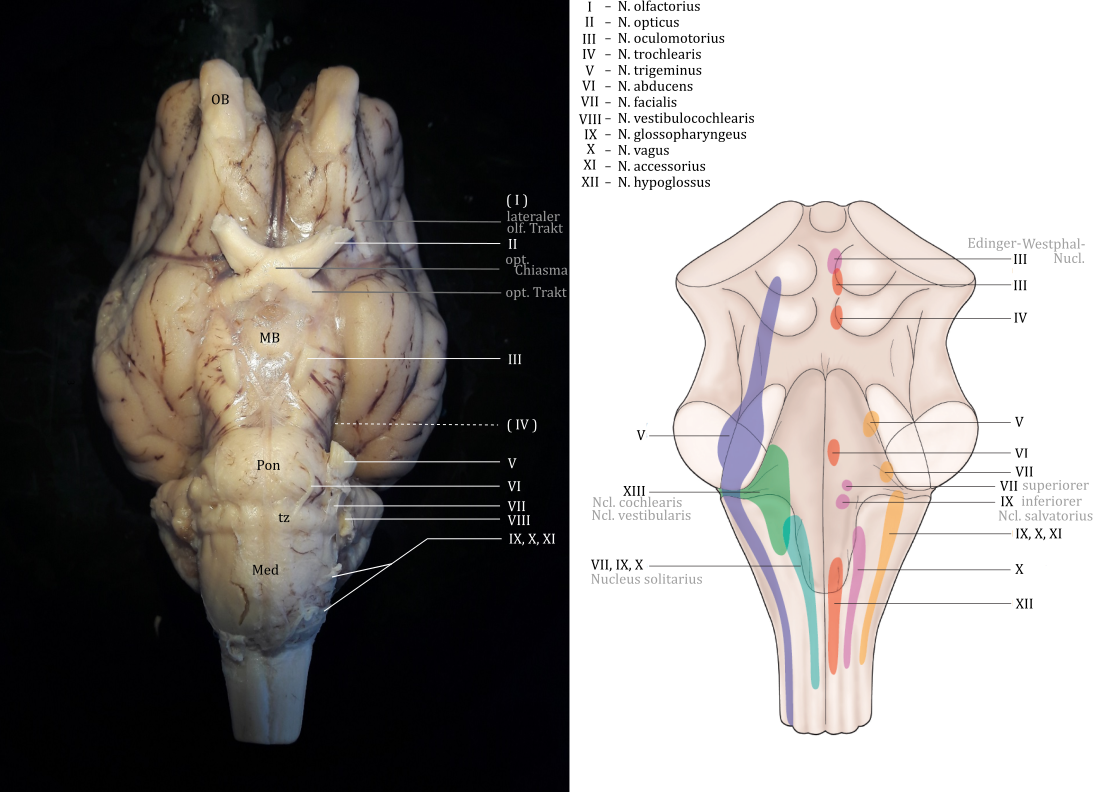
\includegraphics[width=\textwidth]{pictures/Bilder_Jule/Schaf/Aussenansicht/Hirnnerven.png}
    \caption[Hirnnerven Schaf]{\textbf{Hirnnerven Schaf.} \textbf{LINKS:} Ventralansicht des Schafshirns. Gekennzeichnet sind die Hirnnervenkerne. Der Bulbus olfactorius (OB), der Mammillarkörper (MB), der Pons (Pon), der Trapezkörper (tz), sowie die Medulla (Med) sind ebenfalls gekennzeichnet. Da der N. trochlearis nicht sichtbar ist, ist lediglich seine ungefähre Position markiert. \textbf{RECHTS:} dorsale Ansicht des Hirnstamms des Schafs. Markiert sind die Nuclei der Hirnnerven. Dabei sind die sensorischen Kerngebiete links, die motorischen rechts gekennzeichnet. Abbildung nach \textit{Neuroanatomy}, Crossman und Neary \textsuperscript{\cite[Kap.~10]{crossman2014neuroanatomy}}.}
    \label{fig:hirnnerven_schaf}
\end{figure}